\subsection{Instruction Encoding}

In the MIPS32 architecture, all machine instructions are represented
as 32-bit numbers. Throughout this document we will intermittently
dissect these 32-bits into various lengths. We regard the ``upper''
--- or equivalently the ``leftmost'' --- bits as the most significant
bits. Hence, we consider the bit order to be little endian.

In little endian bit notation we denote bit 0 as being the least
significant bit (LSB) and bit 31 as the most significant bit (MSB).

Then, for all MIPS32 instructions we have that the leftmost six bits,
31-26, forms the primary opcode. These bits constitute a field which
are referred to as the \tt{op} field of the instruction.
Depending on the value of the primary opcode there can be an extended
opcode in the rightmost six bits, i.e. bits 0 through 5.  These bits
are referred to as the \funct{} field.\footnote{The decoding of
  the \funct{} field provides details of the required operation
  to the \tt{ALU}.}

Ostensibly, the different fields a MIPS instruction should be divided
into is determined solely by the opcode. The manner in which the bits
are divvied up into fields depends on which instruction format that
the instruction has.

Regardless of the type of the instruction we have that the
\opcode{} field is the uppermost six bits of all MIPS
instructions. Opcode, short for ``operation code'', either identifies
a unique instruction or a \emph{set} of instructions.

While MIPS consists of over a 100 different instructions only 6 bits
are used for the \opcode{}, meaning that the
\opcode{}-field can only be used to differentiate between
$2^6=64$ instructions. 

For R-type instructions an additional 6 bits are used (\textbf{B5-0})
called the ``function'', which serves as a secondary opcode to
identify the instruction. I.e. the tuple

\begin{equation*}
(\opcode{},\ \funct{})
\end{equation*}

is sufficient to \emph{uniquely} identify an R-type instruction.

Other instructions, such as \texttt{bltzal}\footnote{Not an R-type
instruction}, is identified by the tuple

\begin{equation*}
(\opcode{}=1,\ \rt{}=16) \textrm{\hspace{1em}(Remark: base 10)}
\end{equation*}

The MIPS ISA groups its instructions into three
categories:\footnote{Some people consider floating-point and branching
  instructions to be their own respective categories} R-type, I-type, and J-type.

\subsubsection{R-type format}

R-type instructions refer to \emph{register} type instructions. These,
when encoded in machine code, are split into 6 fields of lengths 6, 5,
5, 5, 5, 6 respectively, see ~\autoref{fig:r-type-format-bit-fields}.

\begin{figure}[H]
  % Center the image on the page using makebox  
  \makebox[\textwidth][c]{
    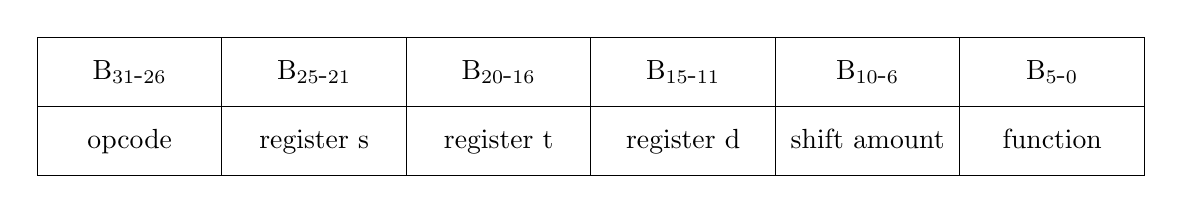
\begin{tikzpicture}[auto,
    every node/.style={rectangle, minimum height=2.5em, text centered, text width=6em, text height=1.5ex, text depth=.25ex},
    field/.style={draw}]
\matrix (m) [ampersand replacement=\&, column sep=-\pgflinewidth, row sep=-\pgflinewidth]
{
\node [field] {$\textrm{B}_{31\textrm{-}26}$}; \&
\node [field] {$\textrm{B}_{25\textrm{-}21}$}; \&
\node [field] {$\textrm{B}_{20\textrm{-}16}$}; \&
\node [field] {$\textrm{B}_{15\textrm{-}11}$}; \&
\node [field] {$\textrm{B}_{10\textrm{-}6}$}; \&
\node [field] {$\textrm{B}_{5\textrm{-}0}$}; \&
\\
\node [field] {opcode}; \&
\node [field] {register s}; \&
\node [field] {register t}; \&
\node [field] {register d}; \&
\node [field] {shift amount}; \&
\node [field] {function}; \&
\\
};
\end{tikzpicture}
%
  } 
  \caption{The bitfields of an R-type format instruction}
  \label{fig:r-type-format-bit-fields}
\end{figure}

For instance, \tt{add} is an R-type instruction, and in
its mnemonic form it looks like

\begin{lstlisting}[style=mips_lst]
add $rd, $rs, $rt
\end{lstlisting}
%$

where \tt{\$rd} refers to some register \tt{d}.

The semantics of the instruction is

\begin{lstlisting}[style=semantics_lst]
R[d] = R[s] + R[t]
\end{lstlisting}

where the addition is signed addition. Hence, \tt{\$rd} is the
target/destination register while the operands \tt{\$rs} and
\tt{\$rt} are the two source registers.\footnote{Notice that the
  mnemonic representation specifies the destination register
  \emph{first} followed by the two source registers but the the actual
  binary format stores the two source registers first, then the
  destination register.}

Certain R-type instructions places certain constraints on its
constituent fields beyond the value of the opcode and the funct
field. Several instructions are only valid if \shamt{} is set to
0, and specifies the shift amount used by shifting instructions such
as \tt{sll} (shift left logical). \tt{clo} (count leading
zeroes) expects both \shamt{} and \tt{rt} to be equal to
zero, and meanwhile \tt{div} (divide with overflow) expects
\rd{} and \shamt{} to be zero.

\subsubsection{I-type format}

I-type stands for "immediate type", and it is decomposed into four
fields. See ~\autoref{fig:i-type-format-bit-fields}.

\begin{figure}[H]
  \makebox[\textwidth][c]{
    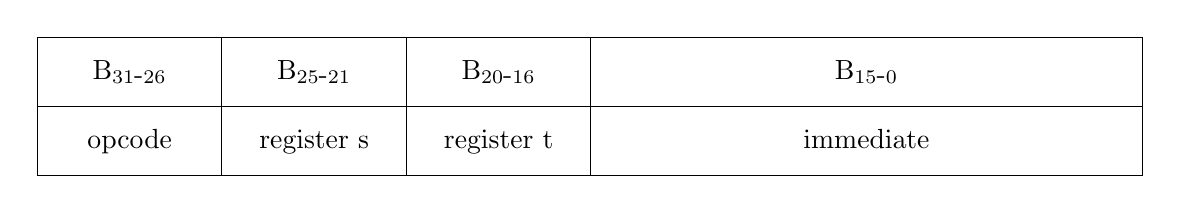
\begin{tikzpicture}[auto,
    every node/.style={rectangle, minimum height=2.5em, text centered, text width=6em, text height=1.5ex, text depth=.25ex},
    field/.style={draw, anchor=west}]
\matrix (m) [ampersand replacement=\&, column sep=-\pgflinewidth, row sep=-\pgflinewidth]
{
\node [field] {$\textrm{B}_{31\textrm{-}26}$}; \&
\node [field] {$\textrm{B}_{25\textrm{-}21}$}; \&
\node [field] {$\textrm{B}_{20\textrm{-}16}$}; \&
\node [field, text width=19.25em] {$\textrm{B}_{15\textrm{-}0}$}; \&
\\
\node [field] {opcode}; \&
\node [field] {register s}; \&
\node [field] {register t}; \&
\node [field, text width=19.25em] {immediate}; \&
\\
};
\end{tikzpicture}
%
  }
  \caption{The bitfields of an I-type format instruction}
  \label{fig:i-type-format-bit-fields}
\end{figure}

The prototypical I-type instruction in its mnemonic form looks as follows,

\begin{lstlisting}[style=mips_lst]
addi $rt, $rs, immed
\end{lstlisting}

In this case, \tt{\$rt} is the destination register, and
\tt{\$rs} is the \emph{only} source register.

The semantics of the \tt{addi} instruction is

\begin{lstlisting}[style=semantics_lst]
R[t] = R[s] + (IR$_{15})^{16}$ IR$_{15\textrm{-}0}$
\end{lstlisting}

where \tt{IR} refers to the instruction register, the register
where the current instruction is stored. \tt{(IR$_{15}$)$^{16}$}
means that bit \textbf{B15} of the instruction register (which is the
sign bit of the immediate value) is repeated 16 times. This is then
followed by \tt{IR$_{15\textrm{-}0}$}, which is the 16 bits of
the immediate value.

Basically, the semantics says to sign-extend the immediate value to 32
bits, add it (using signed addition) to register \tt{R[s]}, and store
the result in register \tt{\$rt}.

For an example,

\begin{lstlisting}[style=mips_lst]
addi $s1, $s2, 100
\end{lstlisting}
%$

stores the value of $(\tt{\$s2} + 100)$ in \tt{\$s1}.

\subsubsection{J-type format}

All jump instructions belong to the J-type format

J-type instructions refer to \emph{jump} type instructions. These,
when encoded in machine code, are split into 2 fields of lengths 6 and
26, respectively. See ~\autoref{fig:r-type-format-bit-fields}.

\begin{figure}[H]
  \makebox[\textwidth][c]{
    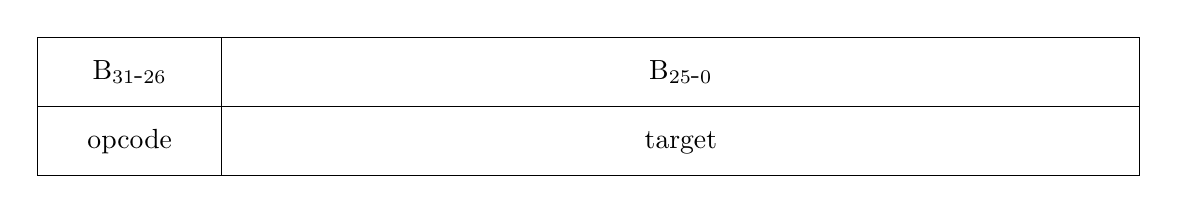
\begin{tikzpicture}[auto,
    every node/.style={rectangle, minimum height=2.5em, text centered, text width=6em, text height=1.5ex, text depth=.25ex},
    field/.style={draw}]
\matrix (m) [ampersand replacement=\&, column sep=-\pgflinewidth, row sep=-\pgflinewidth]
{
\node [field] {$\textrm{B}_{31\textrm{-}26}$}; \&
\node [field, text width=32.5 em] {$\textrm{B}_{25\textrm{-}0}$}; \&
\\
\node [field] {opcode}; \&
\node [field, text width=32.5 em] {target}; \&
\\
};
\end{tikzpicture}
%
  }
  \caption{The bitfields of an J-type format instruction}
  \label{fig:j-type-format-bit-fields}
\end{figure}

For an example the instruction \tt{j} is J-type instruction, and in
its mnemonic form as follows,

\begin{lstlisting}[style=mips_lst]
j target
\end{lstlisting}
%$

\tt{j} is the archetypal jump instruction. In ~\autoref{lst:jump}
``\PC{}'' stands for ``program counter''. The program counter stores
the current address of the instruction that is \emph{currently}
being executed.

In effect, what the \tt{j} instruction does, as shown in
~\autoref{lst:jump}, is re-assign the \PC{} the 32-bit address given
by the upper 4 bits of the \PC{} followed by the 26-bits making up the
target, followed by two zeroes.

\begin{lstlisting}[style=semantics_lst, label={lst:jump}]
PC := PC$_{31\textrm{-}28}$ IR$_{25\textrm{-}0}$ 00
\end{lstlisting}

